\chapter{Probability and statistics}
% TODO missing statistics concepts
% - http://sahilmohnani.wordpress.com/2013/06/02/absolute-mean-deviation/
% - http://sahilmohnani.wordpress.com/2013/06/03/a-multiple-linear-regression-wait-what-did-i-read-that-correctly/
% http://sahilmohnani.wordpress.com/2013/06/03/the-multinomial-and-poisson-distributions/
% - http://sahilmohnani.wordpress.com/2013/06/03/the-chi-square-distribution/
% - Stem-and-leaf plot example http://www.purplemath.com/modules/stemleaf.htm
% - Statistical vs non statistical questions (average vs deterministic)
% - probability models (should probabilities sum to 1)

Probability and statistics are among the most commonly used branches of mathematics. Politicians try to predict the voters opinion of important matters by polling samples of the total population, medical researchers try to infer what percentage of a users of a medicine will be impacted by side effects, economists try to gauge the effectiveness of fiscal policy studying sample data, physics studies dynamic systems, in which the behavior of its part cannot be known in detail but only assigned a probabilities.

The ability to calculate probabilities transformed the practice of statistics, changing it from the mere collection and tabulation of data to the use of data to draw inferences and make informed decisions.

The pundits and pollsters who today tell us who is likely to win the next election make direct use of mathematical techniques developed by Pascal and Fermat. In modern medicine, future-predictive statistical methods are used all the time to compare the benefits of various drugs and treatments with their risks.

In short probability is an enormously useful subject. In spite of its usefulness the formal study of probabilities is rather new branch of matematics. The earlist attempts of describing probability using formal mathematics comes from gambling. The sixteenth century polymath Gerolamo Cardano demonstrated the efficacy of defining odds on games as the ratio of favorable to unfavorable outcome. Later these ideas was picked up and expanded upon by  Pierre de Fermat and Blaise Pascal (1654). In recent years the study of probability and statistics has gained pace as computers allows us to perform studies on and make inference from large samples.

In 1494, in his book Summa de arithmetica, geometrica, proportioni et proportionalita (Everything About Arithmetic, Geometry, and Proportions), Luca Pacioli first put into print the problem that Pascal and Fermat would solve two centuries later. Known as the problem of the unfinished game, it asks how the stakes should be divided when a game of several rounds must be abandoned unfinished. The puzzle is also known as the problem of the points, since rather than counting rounds, we can assign each player points for winning each round.

Suppose two players—call them Blaise and Pierre—place equal bets on who will win the best of five tosses of a fair coin. They start the game, but then have to stop before either player has won. How do they divide the pot?

If each has won one toss when the game is abandoned after two throws, then clearly, they split the pot evenly, and if they abandon the game after four tosses when each has won twice, they do likewise. But what if they stop after three tosses, with one player ahead 2 to 1?.

Pacioli, the man who first wrote about the problem, considered a version in which the game is played until one player has won six rounds, but play is abandoned when the score is 5 to 2. He suggested that the solution is to divide the pot according to the current state of play, namely, 5 to 2, but this reasoning is incorrect as was demonsgrated in 1539 by the itallian polymath Gerolamo Cardano. Cardano noted, correctly, that the apportionment of the pot depended not on how many rounds each player had already won (as Pacioli thought) but on how many each player must still win in order to win the contest.

In this version, the players, Blaise and Pierre, place equal bets on who will win the best of five tosses of a fair coin. We’ll suppose that on each round, Blaise chooses heads, Pierre tails. Now suppose they have to abandon the game after three tosses, with Blaise ahead 2 to 1. How do they divide the pot? The idea is to look at all possible ways the game might have turned out had they played all five rounds. Since Blaise is ahead 2 to 1 after round three, the first three rounds must have yielded two heads and one tail. The remaining two throws can yield H H H T T H T T Each of these four is equally likely. In the first (H H), the final outcome is four heads and one tail, so Blaise wins; in the second and the third (H T and T H), the final outcome is three heads and two tails, so again Blaise wins; in the fourth (T T), the final outcome is two heads and three tails, so Pierre wins. This means that in three of the four possible ways the game could have ended, Blaise wins, and in only one possible play does Pierre win. Blaise has a 3-to-1 advantage over Pierre when they abandon the game; therefore, the pot should be divided 3/4 for Blaise and 1/4 for Pierre.

Today, we are so used to the idea that the future comes with probabilities—the chance that it will rain tomorrow, that house prices will rise over the coming months, that an individual will die within the next five years. people no longer saw the future as completely unpredictable and beyond their control. They could compute the likelihoods of various things’ happening and plan their activities—and their lives—accordingly. In short, we can manage risk.

Cardano’s Liber de ludo aleae (Book of Games of Chance) was published in 1663, In this book he noted

"For example, I can as easily throw one, three or five as two, four or six. The wagers there are laid in accordance with this equality if the die is honest."

thus for the first time formulating what we now call the probability of an event as a fraction: the number of ways the event can occur divided by the total number of possible outcomes. More penetrating, he observed that to obtain the probability of getting a certain outcome on two successive throws, you square the probability of getting it on a single throw. For example, the probability of getting a 6 twice in succession is 1/6 × 1/6 = 1/36. Similarly, the probability of getting an even number twice in succession is 1/2 × 1/2 = 1/4. Extending the reasoning, the probability of getting a 6 three times in a row will be 1/6 × 1/6 × 1/6 = 1/216, and the probability of rolling three even numbers is 1/2 × 1/2 × 1/2 = 1/8. This assumes that the first action does not influence the next—in modern parlance, the two occurrences of the action have to be independent.

For example, the probability of rolling a 6 on the first throw and any even number on the second is 1/6 × 1/2 = 1/12. (If you remove the restriction on the order in which the 6 and an even number occur, there are more possibilities and, accordingly, the probability is bigger. The easiest way to calculate the probability in this case is to do what Fermat did in considering the problem of the points, and enumerate all the favorable outcomes. They are 2-6, 6-2, 4-6, 6-4, 6-6. Since there are 36 possible outcomes altogether, this gives the answer 5/36.)

More tricky is Cardano’s next result: he calculated the probability of throwing a 1 or a 2 with not one die but a pair of dice. The probability of throwing a 1 or a 2 with a single die is 1/3, so the naive intuition is that with two dice, you double your chances—that is, to a probability of 2/3. But as Cardano observed, this is incorrect. The problem is that a 1 or a 2 could come up on both throws, and by adding the two individual probabilities, you would be counting this possibility twice. The probability of not rolling a 1 or a 2 with a single die is 4/6, or 2/3, so the probability of not rolling a 1 or a 2 with two dice is 2/3 × 2/3 = 4/9. Hence, since the probability of rolling something is 1, the probability of rolling a 1 or a 2 must be 1 - 4/9 = 5/9.)


\section{Probability}
Probability is a way of attaching a number that describes the possibility of a certain outcome to events that are fundamentally random. For example a coin toss with a fair coin (a coin that has equal chance of landing on each side) would have $50\%$ chance of heads and 50\% chance of tails.

The probability of a event occurring is calculated in different ways based on the nature of the event at hand, in general we speak of events being simple, compound or complementary

% Excercise when throwing t}o dice is it better to bet on the total die showing 9 or 10

(The first rule tells you that if you throw a die, the odds of getting a 1 or an even number are 1/6 + 1/2 = 2/3; the second rule tells you that when you throw a die twice, the odds of getting a 1 followed by an even number are 1/6 × 1/2 = 1/12.)

\subsection{Simple events}
When finding the probability of an event occurring, we use the formula:
\[
\frac{\text{Number of events that meet constraint}}{\text{Number of equally likely events}}
\]
The following examples illustrate how to calculate simple probability using the above formula
\begin{itemize}
\item A toss of a fair coin have two possible outcomes $\{H,T\}$ so the probability of heads is
$P(H) = \frac{1}{2}$.
\item A toss of a fair die has 6 possible outcomes $\{1, 2, 3, 4, 5, 6\}$ so the probability of the die showing six is $P(6) = \frac{1}{6}$, the probability of getting one or six is $P(1|6) = \frac{2}{6}$ and probability of even number as $P(even) = \frac{3}{6}$
\end{itemize}

\subsection{Compound events}
The way Compound events works is that the likelihood of a series of independent events occurring is the multiplication of the likelihood of each individual event. So, if the probability of you finishing this chapter is $9$ out of $10$ ($9/10$), and the probability of you finishing the next one is $9/10$, the total probability of you finishing both chapters isn't $9/10$: it's $9/10 * 9/10 = 81/100$.

\subsection{Complementary events}
Complementary events are events that add together to equal a whole. For example, if the probability of it raining today were 2/5, the probability of it not raining would be $1 - 2/5 = 3/5$.

\section{Data visualization}
When studying data in order to make better decisions we often start by looking for patterns of behavior. The simplest form of pattern is the number of times a specific data value occurs also known as its frequency. For example when schools create learning plans for classes they analyze frequency of the class grades. Armed with this knowledge special measures can be taken, such as splitting the class into multiple groups to be thought separately.

For example, if four students receives an $F$ in mathematics, then the grade $F$ is said to have a frequency of $4$. The frequency of a data is often represented in a table by arranging data values in ascending order of magnitude with their corresponding frequencies. For example on a $A, B, C, D, F$ grading scale the grades $A, A, B, B, B, C, C, D, F$ produces the following frequency table
\begin{table}[H]
\centering
\begin{tabular}{|l|l|}
\hline
\textbf{Grade} & \textbf{Frequency} \\ \hline
A              & 2                  \\ \hline
B              & 3                  \\ \hline
C              & 2                  \\ \hline
D              & 1                  \\ \hline
F              & 1                  \\ \hline
\end{tabular}
\end{table}
the table above can be easily visualized in a frequency plot, where each dot represents a occurrence of the value below
\begin{figure}[H]
\centering
\begin{tikzpicture}
\begin{axis}[
    symbolic x coords={A,B,C,D,F},
    hide y axis,
    axis x line*=bottom,
    height=4cm,
    width=10cm
]
\addplot+[only marks] plot coordinates
	{(A,1) (A, 2) (B,1) (B,2) (B,3) (C,1) (C,2) (D,1) (F,1)};
\end{axis}
\end{tikzpicture}
\end{figure}
from this frequency plot we can easily deduce that the most common grade in the exam was $B$.

While frequency tables are convenient they often become hard to read if the data set contains more than a handful of observations. For these case we often resort to making a histogram or stem-and-leaf plot for the values.

\subsection{Histograms}
Often data is not repetitive enough for the same value to be repeated enough times to draw conclusions from a frequency table. In these cases we instead split the data into groups and count the frequencies of values within each group. For example if test scores are reassured between $0-100$ we may split the scores $15, 72, 55, 29, 67, 89, 33, 65, 78, 90$ in five groups.
\begin{figure}[H]
\centering
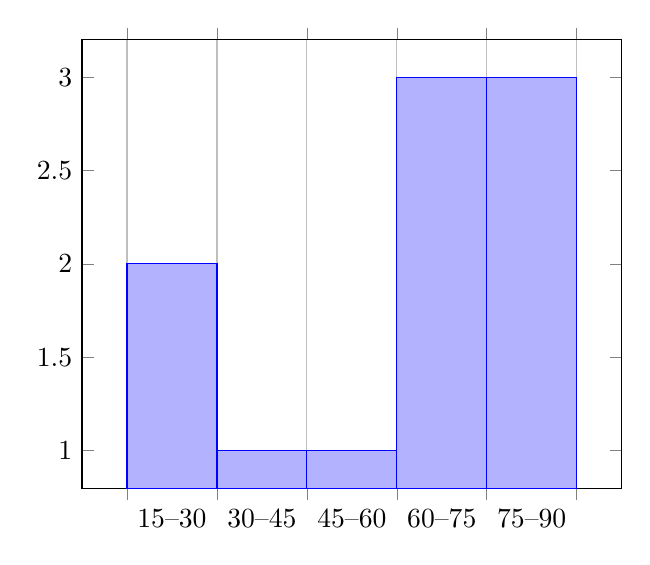
\begin{tikzpicture}
\begin{axis}[
            ybar interval,
            xticklabel=
\pgfmathprintnumber\tick--\pgfmathprintnumber\nexttick
        ]
\addplot+[hist={bins=5}]
            table[row sep=\\,y index=0] {
            data\\
            15\\ 72\\ 55\\ 29\\ 67\\ 89\\ 33\\ 65\\ 78\\ 90\\
            };
\end{axis}
\end{tikzpicture}
\end{figure}

\subsection{Steam and leaf plots}
% http://www.purplemath.com/modules/stemleaf.htm
% TODO describe how its useful to assist in visualizing the shape of a distribution
Steam and leaf plots (The left column of the stem and leaf plot represents the tens place; each number on the right side represents the ones place for the number of pairs of jeans at a department store.)
% TODO draw stem and leaf plot

Next, it must be determined what the stems will represent and what the leaves will represent. Typically, the leaf contains the last digit of the number and the stem contains all of the other digits. In the case of very large numbers, the data values may be rounded to a particular place value (such as the hundreds place) that will be used for the leaves. The remaining digits to the left of the rounded place value are used as the stem.

In this example, the leaf represents the ones place and the stem will represent the rest of the number (tens place and higher).

\subsection{Quartiles}
When using histograms for data analysis we may split the data into any number of groups we deem necessary. This arbitrary split can lead to results that are hard to compare as different researchers may group their data differently. Thus to compare data its useful to group data using a stansafized method, one such method is that of quartiles. With quartiles the data is split into four groups, known as a quartile. Each quartile contains $25\%$ of the total observations. Generally, the data is ordered from smallest to largest with those observations falling below $25\%$ of all the data analysed allocated within the $1st$ quartile, observations falling between $25.1\%$ and $50\%$ and allocated in the $2nd$ quartile, then the observations falling between $51\%$ and $75\%$ allocated in the $3rd$ quartile, and finally the remaining observations allocated in the $4th$ quartile.

When splitting data sets into their quartiles we do so by calculating the boundary values of each quartile known as $Q_1$, $Q_2$ and $Q_3$. Such that

% TODO check this is correct
$1st$ quartile $v \in S where v < Q_1$
$2nd$ quartile $v \in S where v > Q_1 and v < Q_2$
$3rd$ quartile $v \in S where v > Q_2 and v < Q_3$
$4th$ quartile $v \in S where v > Q_3$

to calculate these cuts we use the following method
\begin{enumerate}
    \item Sort data values and find its median (main median)
    \item $Q_1$ is the median of the data left of the main median
    \item $Q_2$ is the main median
    \item $Q_3$ is the median of the data right of the main median
\end{enumerate}

For example the data set $\{0, 1.5, 2.5, 3, 4, 4, 4, 7, 7.5\}$ has the median $4 = Q_2$. The data to the left of the median is $\{0, 1.5, 2.5, 3\}$ which has $2 = Q_1$ as its median. The data to the right is $\{4, 4, 7, 7.5\}$ which has $5.5 = Q_3$ as its median.

% TODO excercise with even number of observations
% 0, 0, 1, 2, 2, 3, 3, 4 (q2 = 2, q1=1/2, q3=3)
% 3, 4, 4, 5, 5, 5, 6, 7 (q2 = 5, q1=4, q3=5,5)
% 7, 9, 9, 10, 10, 10, 11, 12, 12, 14 (q2 = 10, q1=9, q3=12)
% 0, 1, 1, 3, 3, 3, 4, 5, 7 (q2 = 3, q1=1, q3=4,5)

\subsubsection{Five number summary}
% TODO

\subsubsection{Inter quartile range}
The inter quartile range is the range between $Q_3$ ans $Q_1$ or formally $Q_3 - Q_1$

% TODO why is this useful
% TODO excercise with even number of observations

\subsubsection{Box plots}
% TODO explain box plots

\begin{tikzpicture}
  \begin{axis}
    \addplot+[
    boxplot prepared={
      median=1,
      upper quartile=1.2,
      lower quartile=0.4,
      upper whisker=1.5,
      lower whisker=0.2
    },
    ] coordinates {};
  \end{axis}
\end{tikzpicture}

\subsection{Distributions}
% TODO draw examples of the different dsitributions
% TODO (symetrical/asymetrical)
% skewed (skewed to the right = right tailed, skewed to the left = left tailex )
% TODO http://stattrek.com/statistics/charts/data-patterns.aspx clusters, gaps, peeks, outliers
% - peek: value where most observations occur
% - gap: a range of values where no observations occur
% - cluster: a group of observatiins sepearetd from other observatiins by gaps
% - outlier: observations seperated by gaps from the main distribution


\section{Mean, Median and Mode}
Mean, median, and mode are three kinds of "averages".
% TODO describe their usages
\begin{description}
\item [Mean (arithmetic mean)] The sum of numbers divided by the number of numbers e.g. the mean of $\{3, 3, 5, 9, 11\}$ is $(3 + 3 + 5 + 9 + 11)/5 = 6.2$.
\item [Median] The "middle" value of the numbers. To find the median arranging all the observations from lowest to highest and pick the middle one (e.g., the median of $\{3, 3, 5, 9, 11\}$ is $5$). If there is an even number of observations then the median is the mean of the two middle values (the median of $\{3, 5, 7, 9\}$ is $(5 + 7) / 2 = 6$).
\item [Mode] The "mode" is the value that occurs most often. If no number is repeated, then there is no mode. e.g. the mode of $\{3, 3, 5, 9, 11\}$ is $3$. In the data set:
$\{1, 1, 1, 2, 2, 2, 3\}$ we see that $1$ and $2$ both have the most occurrences, so they are both modes.
\item [Range] The "range" is the difference between the largest and smallest values. e.g. the range of $\{3, 3, 5, 9, 11\}$ is $11-3=8$.
\item [Mid-range] the mid-range is the arithmetic mean of the maximum and minimum values in a data set
\[
\textrm{MidRange} = \frac{min(x) + max(x)}{2}
\]
\end{description}

\subsection{Deviation}
% TODO describe usage of and when to use
\begin{description}
    \item [Mean absolute deviation] The mean of the distances of each value from their mean.
\begin{enumerate}
    \item Find the mean of all values
    \item Find the distance of each value from that mean (subtract the mean from each value, ignore minus signs
    \item Then find the mean of those distances
\end{enumerate} For example the Mean Deviation of $3, 6, 6, 7, 8, 11, 15, 16$ is $3.75$ as the mean is $9$ and the distances from this are $6, 3, 3, 2, 1, 2, 6, 7$

\end{description}

\section{Regression}
Regression is the main statistical technique used to quantify the relationship between two or more variables. A regression analysis would show a positive relationship between height and weight, for example. The measure of the accuracy of a regression is called R-squared. A perfect relationship, with no error, would have an R-squared of $1.00$ or $100$. Strong relationships, like height and weight, would have an R-squared of around $70$ percent. A meaningless relationship, like hair color and weight, would have an R-squared of zero.

\section{Random samples}
A random sample of $25\%$ of a schools pupules shoved that 16 pupiles had red hair. Based on the data, what is the most reasonable estimate of the total number of pupiles with red hair on the school?. $25\%$ is the same as $1/4$ of the pupiles at the school so the most resonable estimate is $4$ times the number from the sample $4 \cdot 16 = 62$

\section{Conditional probabilities}
%Index: The Monty Hall Problem
The most famous confusing problem of conditional probabilities is probably the Monty Hall Problem. At the last round of a game show, you’re faced with three curtains. Behind one of the curtains, there is a car, behind the two others there is a goat. You’re asked by the presenter to make a first choice. He then reveals one of the curtains you haven’t chosen which contains a goat. The presenter then gives a chance to change your mind and switch curtain.

\begin{table}[htb!]
\begin{tabular}{|l|l|l|l|}
\hline
\textbf{door 1} & \textbf{door 2} & \textbf{door 3} \\ \hline
stay            & switch          & switch          \\ \hline
switch          & stay            & switch          \\ \hline
switch          & switch          & stay            \\ \hline
\end{tabular}
\end{table}

\noindent that is if its behind dore 1 and you chose door 1 you should stay if you chose door 2 or 3 you shoukd awitch, equally for door two and three. that is you should switch 6 out of 9 times.

% TODO formal math for montey hall.

if you take a card from a deck it has 1/52 chance of bejng the ace of spades. If you flip 50 of the of the remaining 51 cards in the deck and none of them turns out to be the ace of spades then the remaining card now has 51/52 chances to be the ace of spades, that is significanly more likely than our initial draw.

\section{Probability space}
A probability spaces is a way to models processes consisting of states that occur randomly. For example in a deck of 52 cards the sample space is a 52-element set, as each card is a possible outcome. Since there can be many outcomes (even infinitely many), outcomes elements are grouped into sets which are called "events. For our deck of cards, possible events may include
\begin{description}
\item [- The 5 of Hearts] (1 element),
\item [- A King] (4 elements),
\item [- A Face card] (12 elements),
\item [- A card] (52 elements).
\end{description}
More formally an event, is any subset of the sample space we like to consider in our model, including the empty set (an impossible event, with probability zero) and the sample space itself (a certain event, with probability one).

\noindent To sum up a probability space consists of three parts
\begin{itemize}
\item The sample space $\Omega$ which is a set of all possible outcomes.
\item The $\sigma$-algebra $\mathcal{F}$ which is a collection of the events we would like to consider.
\item The probability measure $P$ which is a function returning an event's probability $P: F \rightarrow [0,1]$.
\end{itemize}

For example if the experiment consists of just one flip of a perfect coin, then the outcomes are either heads or tails: $\Omega = {H, T}$. The $\sigma$-algebra $\mathcal{F} = 2^{\Omega}$ contains $2^2 = 4$ events, namely:
\begin{itemize}
\item $\{H\}$ – "heads"
\item $\{T\}$ – "tails",
\item $\{\}$ – "neither heads nor tails"
\item $\{H,T\}$ – "either heads or tails"
\end{itemize}
So, $\mathcal{F} = \{\{\}, \{H\}, \{T\}, \{H,T\}\}$. Since there is a fifty percent chance of tossing heads, and fifty percent for tails the probability measure in this example is $P(\{\}) = 0, P(\{H\}) = 0.5, P(\{T\}) = 0.5, P(\{H,T\}) = 1$.

\subsection{Random variable}
A random variable (or stochastic variable) is a variable whose value is subject to variations due to chance. A random variable's possible values might represent the possible outcomes of a yet-to-be-performed experiment

The mathematical function describing the possible values of a random variable and their associated probabilities is known as a probability distribution. Random variables can be discrete, that is, taking any of a specified finite list of values; or continuous, taking any numerical value in an interval.

%\section{Propability distributions}
%\subsection{Poison distribution}
%\subsection{Binomial distribution}
%\subsection{Negative binomial distribution}
%\subsection{Compound distributions}
%\subsection{Normal distribution}
%\subsection{Gamma distribution}
%\subsection{Lognormal distribution}
%\subsection{Pareto distribution}
%\subsection{Chi-squared distribution}

\section{Exercises}

\begin{ExerciseList}

% MEAN, MEDIAN and MODE excercises

\Exercise A gardening store offers $4 $ different flowers $\{f_1, f_2, f_3, f_4\}$ tand $4$ different types of pots $\{p_1, p_2, p_3, p_4\}$, how many different arrangement of pot and plant can you make
\Answer Each of the four plants can be placed in four different pots yielding $4 \cdot 4 = 16$ possible arrangements

\Exercise If you role a fair six sided die and a fair four sided die what is the probabilityb that neither will shown one
\Answer $P(\text{six sided not not one}) \cdot P(\text{four sided not not one}) = 5/6 * 3/4 = 5/8$

\Exercise You are given two dice to roll. One is black with six sides; the other is white with four sides. For a given roll, what is the probability the black die is even and the white die is $2$
\Answer $P(\text{even black die}) \cdot P(\text{white die is 2}) = 3/6 * 1/4 = 3/24$

\Exercise You are going to randomly select a marble from a bag of marbles that contains $3$ blue marbles, $4$ green marbles, and $5$ red marbles. What is $P(\text{blue marble})$
\Answer $P(blue marble) = \frac{\text{number of blue marbles}}{\text{total number of marbles}} = 3/12 = 0.25$

\Exercise A store offers sells four types of cloth: shirts, pants, socks and hats and offers each in three colors orange", purple and blue. If you randomly pick the piece of clothing and the color, what is the probability that you'll end up with an orange hat
\Answer $1/3 \cdot 1/4 = 1/12$

\Exercise If you flip a fair coin $1200$ times. What is the best prediction for the number of times that the coin will land heads up?
\Answer $1/2 \cdot 1200 = 600$

\Exercise If you toss a fair die $180$ times what is the best prediction of the number of times you will get more than $4$
\Answer $2/6 \cdot 180 = 60$

\Exercise You've decided to flip $3$ coins, how many possible outcomes are there.
\Answer There are two possible outcomes for the first flip, two for the second and two for the thrid, thus $2 \cdot 2 \cdot 2 = 8$ possible outomes.

\Exercise If a pirate and a navy boat fires at each other simultanously and the navy boat has $3/5$ probability of a hit and the pirate $1/3$. What is then the probability that the navy hits and the pirate misses ?
\Answer Our scenario has probability $P(\text{navy hits}) * P(\text{pirate misses})$ which is $3/5 \cdot (1 - 1/3) = 3/5 \cdot 2/3 = 6/15 = 2/5$.

\Exercise In a class of $7$, there are $3$ students who have red hair. If the teacher randomly chooses $2$ students, what is the probability that neither of them have red hair.
\Answer there is a $4/7$ chance that the first student is not a red hair and $3/6$ chance that the second student is not so $4/7 * 3/6 = 12/42 = (2*2*3)/(2*3*7) = 2/7$.

\Exercise Three dice are thrown simultaneously. Find the probability that:
\Question All show distinct faces
\Question Two of them show the same face
\Answer TODO % http://math.stackexchange.com/a/470067

\end{ExerciseList}
